\documentclass[11pt, a4paper, twocolumn]{article}

\newcommand{\getTitle}{Principles of Object-Oriented Programming Languages: Language Comparison}
\newcommand{\getAuthor}{Mathijs Saey}
\newcommand{\getFullTitle}{Principles of Object-Oriented Programming Languages: \\ Language Comparison}
\newcommand{\getFullAuthor}{Mathijs Saey, 94451,  \\ mathsaey@vub.ac.be, \\ 1st Master of Science in Applied Sciences and Engineering: \\ Computer Science}

\newcommand{\mytilde}{\raise.17ex\hbox{$\scriptstyle\mathtt{\sim}$}}

%Packages
\usepackage{color}
\usepackage{graphicx} 
\usepackage{listings}
\usepackage{longtable}

%Bibliography
\usepackage{biblatex}
\addbibresource{references.bib}

%Hyperref + pdf meta info
\usepackage[hidelinks]{hyperref}

\hypersetup{
 	pdfauthor={\getAuthor},
 	pdftitle={\getTitle},
 	pdfkeywords={VUB, Object-oriented, C++, Objective-C},
 	pdfproducer=pdfLatex,
 	pdfcreator=Sublime Text 2,
}

%Extra colors
\definecolor{dkgreen}{rgb}{0,0.6,0}
\definecolor{gray}{rgb}{0.9,0.9,0.9}
\definecolor{mauve}{rgb}{0.58,0,0.82}

% Listing settings
\lstset{language=C++,
	basicstyle=\scriptsize,
	backgroundcolor=\color{gray},
	commentstyle=\color{dkgreen},
	numberstyle=\scriptsize\color{black},
	keywordstyle=\color{blue},
	morekeywords={@interface, @end, @protocol, @implementation, alloc, init, import, id},
	numbers=left,
	xleftmargin=9pt,
	framexleftmargin=9pt,
	breaklines=true,
	numbersep=1pt,
	tabsize=2}


\begin{document}

%Options
\setlength{\parindent}{0pt}
\setlength{\parskip}{1ex}

%Title + table of contents
\onecolumn 
%Title page
\title{\getTitle}
\author{\getFullAuthor}
\date{\today}
\maketitle

%Vub Logo
\begin{figure}[!]
\centerline{

\includegraphics[scale=0.2]{files/vub_logo.jpg}}
\end{figure}
\newpage
\tableofcontents
%Content

\section{Introduction}
\subsection{About}
This paper is written for the Principles of Object Oriented Languages course at the VUB. The goal of this paper is to compare the object oriented properties of 2 languages. 

\subsection{Languages}
Objective-C and C++ were chosen for this purpose, these languages are both strict supersets of C, but have a very different appraoch on object oriented features. C++ is focussed towards run-time efficieny and static type checking \cite{CPdesc}; while Objective-C tries to do things dynamically whenever this is possible \cite{OCRPG}.

Both languages were compiled with llvm-gcc, with the following version info: "i686-apple-darwin11-llvm-gcc-4.2 (GCC) 4.2.1 (Based on Apple Inc. build 5658) (LLVM build 2336.11.00)". In the case of Objective-C, the \textit{Foundation} runtime was used (received by appending -framework Foundation to the standard gcc compile instruction). Finally, all of the code files and their respective makefiles can be found at \url{https://github.com/mathsaey/POOL-Paper} in case of any issues.

\subsection{Structure}
At first, the general properties of both languages will be compared (such as access levels and the typing system). Afterwards, we will discuss the language features that are unique to each language and attempt to explain their absence in the other language.

\section{General properties}
\label{sec:general}

\subsection{Type system}
\label{sec:types}

Objective-C and C++ are both strict supersets of C, so it should come as no surprise to a reader familiar with C that both languages are statically typed. This is not entirely true for objective-C though. Objective-C introduces the \textit{id} type, this type can be a pointer to any object. This effectively means that an Objective-C programmer can use dynamic and static typing next to each other. 

This seemingly small difference already leads to some differences between our languages. This difference is mainly apparant when we need to create a function that can accept any type of object. An Objective-C programmer faced with such a problem simply uses a variable with the id type, the programmer can now send messages to the variable or store it internally without worrying about the type.

C++ introduces the concept of templates to deal with this. A programmer can create generic functions and classes using the template system. To use one of these functions we just provide the type of the variable to the class and the compiler will generate a version of that class that can handle the variable. This does mean that functions and classes that are built using templates can only accept the types that they were instantiated with. For instance, if we create a vector that contains strings in C++ then that vector will only be able to hold strings. An array in Objective-C on the other hand, can hold any variable with the id type, the type that can point to anything. Listings \ref{cp:typ} and \ref{oc:typ} show this array example in code.

\subsection{Access modifiers}
\label{sec:access}
\subsubsection{Member Variables}
Objective-C and C++ both support \textit{public}, \textit{protected} and \textit{private} member variables. Public variables are visible to anyone, while private variables are visible to the class (not the instance!) to which they belong. Protected variables are visible to the class to which they belong and any subclass of this class. It's important to note that an instance of class A can still access the private variables of another instance of A. This is possible in Objective-C and in C++.

It's also worth mentioning that Objective-C does allow you to access a protected variable outside of the class. The compiler generates a warning, but still allows you to do this. The following warning is shown: 
\textit{"warning: instance variable ‘b’ is @protected; this will be a hard error in the future"}.
Furthermore, the reflective features of Objective-C still allow a programmer to access private instance variables. This is because access modifiers are checked at compile time and not at runtime. Reflection is mentioned in greater detail in section \ref{sec:reflection}

\subsubsection{Methods}
Member variables have the same access modifier structure in C++ and Objective C, this is not the case for methods. C++ uses the same conventions for all members, methods and variables all use the same private, protected, public access modifiers. This is not the case in Objective-C. 

In Objective-C any class can accept any message; the runtime will lookup the method in the class's \textit{dispatch table}\cite{OCRPG}[Messaging], if the class has a method that matches, then the method will be executed, if it doesn't then an exception is raised. The only way to "hide" a method from the outside world in Objective-C is not including it in the class's interface. Doing this will let the compiler raise a warning when this method is called outside the class implementation. However, it's still possible for the outside world to trigger the method by sending the correct message.

\subsection{Polymorphism}
\label{sec:polymorphism}

Objective-C and C++ both support polymorphism. Polymorphism allows different classes to react in different ways to the same message/method call. In C++ we can create a noisemaker class that has a \textit{makeNoise} method. Another method, print, can accept any subclass of noisemaker and returns the value of makeNoise to the user (listing \ref{cp:pol}.). 
Thus polymorphism allows us to treat a given object (that is a subclass of noisemaker) in the same way while still receiving the class-specific behaviour.

We created the same example in Objective-C (listing \ref{oc:pol}). Note how both of our noisemaker objects don't need to share a parent to show the same behaviour? This is the id type allowing us to refer to any type, combined with the fact that an object in Objective-C can accept any message. In C++, calling an unknown message will result in a compile error. Giving 2 objects a common superclass is the only way to obtain polymorphism in C++. 

In Objective-C we use a \textit{protocol} (more on this in section \ref{sec:protocol}) to indicate that car and sheep both implement the makeNoise method. It's worth noting at this point that this example would still work without the noisemaker protocol. The protocol merely allows the compiler to generate a warning if car or sheep do not implement the makenoise protocol. 

\subsection{Inheritance}
\label{sec:inheritance}
Objective-C uses a relatively simple, single inheritance model. An object that receives a message for which it has no methods simply checks if it's superclass implements this method. Instance variables of the super class will keep their access level. An interesting property is that Objective-C doesn't allow overriding variables, adding a variable with name 'x' will raise a compiler error if a superclass already has a variable named 'x'.

This problem does not exist in C++, adding a variable that has already been defined raises no error. Accessing the variable of the superclass is simply achieved by prefixing the variable name with "\textit{superClassName::}". The same prefix is used to access functions of a superclass. This method has to be used since C++ has no \textit{super} keyword. This might seem strange at first, but this feature allows a C++ class to inherit from multiple classes. This feature is called "\textit{explicit qualification}". Using explicit qualification solves any possible ambiguities when inheriting from multiple parents. 

\begin{figure}[h]
\centerline{
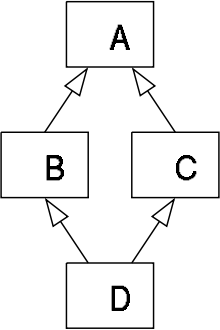
\includegraphics[scale=0.5]{files/diamond.png}}
\label{img:diamond}
\caption{The diamond problem illustrated (source: Wikipedia)}
\end{figure}

A common multiple inheritance problem is the \textit{diamond problem}. This problem occurs when a class D inherits from classes B and C that have a common parent A. If D calls a method defined in A that has different behaviour in B and C then which version of the method will be called? C++ solves this problem by keeping a sperate instance of A for both B and C, explicit qualification ensures that the correct version of the method is called. If B and C inherit A \textit{virtually}, then the compiler ensures that only one A object is constructed.

A C++ class does not inherit access rights in the same way that Objective-C does. The access right of the inherited class has to be explicitly mentioned. This access right then transfers to the members of that superclass. If the inherited class is declared public, then the access rights remain the same. If the inherited class is declared protected, then every public member of the superclass is protected in the subclass. If the inherited class is declared private, then every member of the superclass is private in the subclass.

\subsection{Constructors and Destructors}
\label{sec:constructor}
C++ constructors are normal methods with no return type and the class name as their signature. Method overloading (see section \ref{sec:overloading}) allows the definition of multiple constructors. Destructors in C++ are declared in a similar way, however, a destructor cannot accept any arguments and is named "\textit{\mytilde{}Classname()}". A destructor will be automatically called right before deleting an object.

The Objective-C language has no mandatory constructors or destructors. Constructing and deconstructing an object generally happens by overriding a few methods inherited from NSObject. These methods are listed here: 
\begin{itemize}
\item \textbf {alloc} Alloc allocates the space that the object needs.
\item \textbf {init} Init inialises the necessary instance variables.
\item \textbf {dealloc} Dealloc releases all the instance variables.
\end{itemize}

Note that nothing prevents an Objective-C programmer from creating his own alloc, init or dealloc that don't derive from NSObject directly or indirectly. For instance, a programmer that wants to implement the singleton pattern generally overrides alloc to ensure that an object is only created when he wants it.
Initialisers generally derive from NSObject's init at some point (via a call to super init). Conventions dictate that initialisers start with init. Multiple initialisers are simply constructed by creating different methods, note that - unlike in C++, where a constructor has no return type or statement - an initisialiser should return itself after instantiating the necessary instance variables.

\section{Lanaguage-Specific \-Features}
\subsection{Objective-C}
\subsubsection{Protocols}
\label{sec:protocol}

\subsubsection{Categories}
\label{sec:categories}

\subsubsection{Message Forwarding}
\label{sec:message}

\subsubsection{Reflection}
\label{sec:reflection}

\subsubsection{Metaclasses}
\label{sec:meta}

\subsection{C++}
\subsubsection{Method Overloading}
\label{sec:overloading}

\subsubsection{Namespaces}
\label{sec:namespaces}

\subsubsection{Abstract Classes}
\label{sec:abstract}

\subsubsection{Friend Classes}
\label{sec:friend}

\subsubsection{Inner Classes}
\label{sec:inner}

\section{Conclusion}

%Metaclasses
%Everythingisanobject?       

% Pure virtual classes vs protocols
% Echte abstracte klases zijn er niet in obj-c. C++ heeft geen protocol alternatief
% Meerder @interface van zelfde klasse mogelijk? => Categorien
% nested class => in de implementatie file zetten (zoals private category)
% friend classes emuleren via category

%forwarding voor multiple inheritance? => maakt het mogelijk om een single method te inheriten

%In Objective-C, all methods are virtual. Hence, the virtual keyword does not exist and has no equivalent.

% constructors, destructors

%Bibliography
\printbibliography[heading = bibnumbered]

\section{Code Listings}
\lstinputlisting[label=cp:typ,language=C++,caption={Templates and static typing in C++}]{../C++/Types.cpp}
\lstinputlisting[label=oc:typ,caption={Objective-C using Dynamic and Static typing}]{../objC/Types.m}

\lstinputlisting[label=cp:acc,language=C++,caption={Access rights in C++}]{../C++/Access.cpp}
\lstinputlisting[label=oc:acc,caption={Access rights in Objective-C}]{../objC/Access.m}

\lstinputlisting[label=cp:pol,language=C++,caption={Polymorphism in C++}]{../C++/Polymorphism.cpp}
\lstinputlisting[label=oc:pol,caption={Polymorphism in Objective-C}]{../objC/Polymorphism.m}

\lstinputlisting[label=cp:inh,language=C++,caption={Inheritance in C++}]{../C++/Inheritance.cpp}
\lstinputlisting[label=cp:min,language=C++,caption={Multiple inheritance in C++}]{../C++/MultipleInheritance.cpp}
\lstinputlisting[label=oc:inh,caption={Inheritance in Objective-C}]{../objC/Inheritance.m}


\end{document}
